\chapter{Elektrodinamika}

\begin{defn}[Elektrodinamika]
  Mokslas apie ypatingos materijos rūšies – elektromagnetinio lauko,
  sukeliančio įelektrintų kūnų arba elektringųjų dalelių sąveiką,
  – savybes ir dėsningumus.
\end{defn}

\section{Elektrostatika}

\begin{defn}[Elektrostatika]
  Elektrodinamikos skyrius, kuriame nagrinėjami nejudančių elektros
  krūvių sąveikos dėsniai.
\end{defn}

Gamtoje pasitaiko dviejų rūšių krūviai: teigiami ir neigiami.
\begin{defn}[Elektronas]
  Mažiausia stabili neigiamo krūvio elektringoji dalelė. Jos masė yra
  $9,1 \cdot 10^{-31}$ kg.
\end{defn}
\begin{defn}[Protonas]
  Mažiausia stabili teigiamo krūvio elektringoji dalelė. Jos masė yra
  $1,672 \cdot 10^{-27}$ kg.
\end{defn}
Jų abiejų (elektrono ir protono) krūvis absoliučiuoju didumu yra
vienodas ir yra lygus:
\begin{equation*}
  |e| = 1,6021892(46) \cdot 10^{-19} C
\end{equation*}

\subsection{Krūvių sąveika}

\begin{defn}[Kulono dėsnis]
  Dviejų taškinių nejudančių įelektrintų kūnų sąveikos jėga vakuume
  yra tiesiog proporcinga krūvių modulių sandauga ir yra atvirkščiai
  proporcinga atstumo tarp jų kvadratui:

  \begin{equation}
    F = k \cdot \frac{|q_{1}| \cdot |q_{2}|}{r^{2}}
    \label{eq:kulono_desnis}
  \end{equation}
  čia:
  \begin{description}
    \item[$q_{1}$] – pirmojo kūno krūvis;
    \item[$q_{2}$] – antrojo kūno krūvis;
    \item[$r$] – atstumas tarp krūvių;
    \item[$k$] – Kulono dėsnio koeficientas,
      $k = \frac{1}{4 \pi \varepsilon_{0}} =$
      $9 \cdot 10^{9} \frac{N \cdot m^{2}}{C^{2}}$
      ($\varepsilon_{0}$– elektrinė konstanta, $\varepsilon_{0} \approx $
      $8,85 \cdot 10^{-12} \frac{C^{2}}{N \cdot m^{2}}$).
  \end{description}

  Jei bandymas vyksta ne vakuume, tai:
  \begin{equation*}
    F =
      \frac{1}{4 \pi \varepsilon_{0}} \cdot
      \frac{q_{1}q_{2}}{\varepsilon r^{2}}
  \end{equation*}
  čia:
  \begin{description}
    \item[$\varepsilon$] – aplinkos dielektrinė skvarba, kuri yra lygi
      krūvį vakuume veikiančios jėgos ir jėgos veikiančios
      aplinkoje santykiui:
      $\varepsilon = \frac{F_{\t{vakuume}}}{F_{\t{aplinkoje}}}$.
  \end{description}
\end{defn}

\begin{defn}[Kulonas]
  Krūvis, kuris prateka per vieną sekundę laidininko skerspjūviu, kai
  srovės stiprumas yra vienas amperas:
  \begin{equation*}
    1 C = 1A \cdot 1s
  \end{equation*}
\end{defn}

\begin{defn}[Elektrinio lauko stipris]
  \begin{equation*}
    \vec{E} = \frac{\vec{F}}{q}
  \end{equation*}
  čia:
  \begin{description}
    \item[$F$] – jėga, veikianti taškinį krūvį;
    \item[$q$] – taškinis krūvis.
  \end{description}
  Elektrinio lauko stipris matuojamas $\frac{N}{C}$ arba $\frac{V}{m}$.
\end{defn}

\subsection{Kažkas neaiškaus}

\begin{defn}[Elektrostatinė indukcija]
  Laidininko įsielektrinimas dėl išorinio elektrinio lauko poveikio.
\end{defn}

FIXME Išsiaiškinti kas per velnias yra šitai.
Žr.: \url{http://en.wikipedia.org/wiki/Electric_displacement_field}
Žr.: \url{http://www.scritube.com/limba/lituaniana/Fizikos-formuli-rinkinys11515191913.php}

Gauso teorema:
\begin{equation*}
  \oint _{S} \vec{E} \cdot d \vec{S}
  = \frac{\sum_{i}q_{i}}{\varepsilon_{0}}
\end{equation*}
čia:
\begin{description}
  \item[$\oint_{S}\vec{E} \cdot d\vec{S}$] – elektrostatinio lauko stiprio
    vektoriaus srautas per bet kokį uždarą paviršių,
  \item[$\sum _{i} q_{i}$] – to paviršiaus apribotas krūvis.
\end{description}

\begin{description}
  \item[$\vec{D}$] – elektrostatinė indukcija.
\end{description}
\begin{align*}
  \vec{D} &= \varepsilon_{0} \varepsilon \vec{E}
\end{align*}

\begin{defn}[Elektrinio lauko srautas]
  \begin{equation}
    \Phi = \vec{E} \cdot \vec{S} \cdot \cos \alpha
    \label{def:srautas}
  \end{equation}
  \begin{description}
    \item[$\vec{S}$] – plotas (pseudo vektorius, kryptis sutampa su
      normalės kryptimi);
    \item[$\vec{E}$] – elektrinio lauko stipris.
  \end{description}
\end{defn}

FIXME Išsiaiškinti.
Žr.: \url{http://en.wikipedia.org/wiki/Maxwell's_equations}
\begin{align*}
  \Psi &= \vec{D} \vec{S} = \sum _{i=1} ^{n} q_{i} \\
  \Phi &= \oint_{S} \vec{E} d \vec{S} = 
    \frac{1}{\varepsilon_{0}} \int _{v} \rho dv \\
  \delta A &= \vec{F} \cdot \vec{d} \cdot r =
    q \cdot \vec{E} \vec{d} r = -d W p
\end{align*}

\subsection{Energija}

Iš mechanikos kurso turime, kad darbas yra jėgos ir kelio sandaugai:
\begin{equation}
  A = F \cdot s
  \label{eq:mechanika:darbas}
\end{equation}
čia:
\begin{description}
  \item[$A$] – jėgos atliktas darbas;
  \item[$F$] – kūną veikusi jėga;
  \item[$s$] – kūno nueitas kelias.
\end{description}

Kadangi žinome, kad taškinį krūvį elektriniame lauke veikianti jėga
yra lygi $qE$, tai galime apskaičiuoti elektrinių jėgų atliktą darbą:
\begin{align*}
  F
  &= Fs \\
  &= qEs \\
\end{align*}
Tarkime, kad taškinis krūvis buvo atstumu $d_{1}$ nuo elektrostatinį
lauką kuriančio šaltinio ir pasislinko į $d_{2}$. Tada elektrostatinių
jėgų atliktas darbas yra:
\begin{align*}
  A
  &= qEs \\
  &= qE\left( d_{2} - d_{1} \right) \\
  &= qEd_{2} - qEd_{1} \\
\end{align*}
Iš mechanikos taip pat žinome, jog darbas yra lygus kūno energijos 
pokyčiui: $A = E_{2} - E_{1}$. Pagal analogiją galime pažymėti, kad
krūvio potencinė energija yra:
\begin{equation*}
  W_{p} = qEd
\end{equation*}
čia:
\begin{description}
  \item[$W_{p}$] – krūvio potencinė energija;
  \item[$q$] – krūvio dydis;
  \item[$E$] – elektrinio lauko stipris;
  \item[$d$] – atstumas.
\end{description}

Dabar galime apibrėžti elektrostatinio lauko potencialą:
\begin{defn}[Elektrinio lauko potencialias]
  Potencialas yra skaliarinis fizikinis dydis, lygus krūvio potencinės
  energijos ir to krūvio santykiui:
  \begin{align*}
    \varphi &= \frac{Wp}{q} & \text{vienam taškui} \\
    \varphi &= \sum ^{n} _{i=1} \frac{q_{i}}{4 \pi \varepsilon_{0} r} 
      & \text{taškų sistemai}.
  \end{align*}
\end{defn}

Darbas perkeliant krūvį iš taško su potencialu $\varphi_{1}$ į tašką
su potencialu $\varphi_{2}$ lygus:
\begin{equation*}
  A_{1,2} = q \cdot (\varphi_{1} - \varphi_{2})
\end{equation*}

Potencialų skirtumas dar vadinamas įtampa:
\begin{align*}
  U
  &= \varphi_{1} - \varphi_{2} \\
  &= \frac{A}{q} \\
\end{align*}
čia:
\begin{description}
  \item[$U$] – įtampa;
  \item[$\varphi_{1}$] – pradinio taško potencialas;
  \item[$\varphi_{2}$] – galinio taško potencialas;
  \item[$A$] – krūvio perkėlimo darbas;
  \item[$q$] – krūvis.
\end{description}

Įtampos matavimo vienetai:
\begin{align*}
  1 V = \frac{1 J}{1 C}
\end{align*}
čia:
\begin{description}
  \item[$1 V$] – vienas voltas;
  \item[$1 J$] – vienas džaulis;
  \item[$1 C$] – vienas kulonas.
\end{description}

Vienas elektron-voltas:
\begin{align*}
  1 eV
  &= 1,6 \cdot 10^{-19} C \cdot 1 V\\
  &= 1,6 \cdot 10^{-19} J
\end{align*}

\subsection{Dielektrikai}

\begin{defn}[Dielektrikai]
  Medžiagos, kurios prastai praleidžia elektros srovę.
\end{defn}

Pagal molekulių sandarą dielektrikai skirstomi į:
\begin{description}
  \item[poliniai dielektrikai] – tie, kurių teigiamų krūvių ir neigiamų
    krūvių pasiskirstymo centrai nesutampa;
  \item[nepoliniai dielektrikai] – tie, kurių normaliomis teigiamų
    ir neigiamų krūvių pasiskirstymo centrai sutampa (įnešus nepolinius
    dielektrikus į elektrinį lauką, jų teigiamų ir neigiamų krūvų
    centrai pasislenka į priešingas puses ir todėl juos toliau
    galima nagrinėti lygiai taip pat, kaip ir polinius dielektrikus).
\end{description}

Polines molekules galima apytiksliai nagrinėti, kaip elektrinius dipolius.

\begin{defn}[Elektrinis dipolis]
  Du skirtingų ženklų, bet vienodo modulio, taškiniai krūviai,
  esantys $l$ atstumu vienas nuo kito. Pagrindinė elektrinio dipolio
  charakteristika yra jo dipolinis elektrinis momentas:
  \begin{align*}
    \vec{p_{i}} &= q \cdot \vec{l}
  \end{align*}
  čia:
  \begin{description}
    \item[$p_{i}$] – dipolinis elektrinis momentas;
    \item[$q$] – teigiamo (arba neigiamo) poliaus krūvio didumas;
    \item[$l$] – atstumas tarp krūvių.
  \end{description}
\end{defn}

Įnešus polinį dielektriką į elektrinį lauką, dėl Kulono jėgos atsiranda
sukamasis momentas:
\begin{equation*}
  M = p_{i} \cdot E \sin \alpha
\end{equation*}
čia:
\begin{description}
  \item[$\vec{p_{i}}$] – molekulės dipolinis elektrinis momentas;
  \item[$\vec{E}$] – elektrinio lauko stipris;
  \item[$\alpha$] – kampas tarp vektorių $\vec{p_{i}}$ ir $\vec{E}$.
\end{description}
Dipoliai orientuojasi ir atsiranda dielektriko savasis elektrinis
laukas, kurio kryptis yra priešinga išoriniam. Todėl dielektriko
elektrostatinio lauko stiprumas yra $\varepsilon$ kartų mažesnis
nei vakuumo:
\begin{equation*}
  E = \frac{E_{0}}{\varepsilon}
\end{equation*}
čia:
\begin{description}
  \item[$E$] – elektrinio lauko stiprumas dielektrike;
  \item[$E_{0}$] – elektrinio lauko stiprumas vakuume;
  \item[$\varepsilon$] – aplinkos dielektrinė skvarba.
\end{description}
Dielektriko poliarizacijos vektorius (poliarizuotumas):
\begin{equation*}
  \vec{P} = \frac{1}{V} \sum _{i=1} ^{N} \vec{p_{i}}
\end{equation*}
čia:
\begin{description}
  \item[$N$] – dipolių skaičius tūryje $V$;
  \item[$\vec{p_{i}}$] – i-ojo dipolio elektrinis momentas.
\end{description}

\subsection{Poliarizacijos histerezė}

\begin{defn}[Histerezė]
  Objekto fizikinės būsenos nevienareikšmė priklausomybė nuo fizikinio
  dydžio, apibūdinančio išorines sąlygas. (DLKŽ)
\end{defn}

\begin{defn}[Histerezė]
  Pasekmės atsilikimas nuo ją sukėlusios priežasties; ankstesnių sąlygų
  vėlesnis veikimas. (DLKŽ)
\end{defn}

\begin{defn}[Poliarizacijos histerezė]
  FIXME

  Vyksta feroelektrikuose, jų viduje poliarizuojantis turinčioms dipolinį
  momentą sritelėms, vadinamoms domenais. Šis reiškinys pasižymį
  dvejomis išskirtinėmis savybėmis:
  \begin{itemize}
    \item feroelektrikas nepraranda poliarizacijos, panaikinus išorinį
      elektrinį lauką;
    \item feroelektrikas gali būti poliarizuotas dviem kryptimis.
  \end{itemize}
  \ref{fig:histereze} paveikslėlyje pavaizduota kreivė $P = f(E)$ vadinama 
  histerezės kilpa, o tokia poliarizuotumo priklausomybė – dielektrine
  histereze.
\end{defn}

\begin{figure}[H]
  \begin{center}
    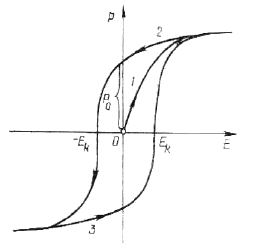
\includegraphics[height=0.5\textwidth]{images/histereze.png}
  \end{center}
  \caption{Histerezės kilpa}
  \label{fig:histereze}
\end{figure}

Pjezo efektas – spaudžiant medžiagą, turinčią dipolių, dipoliai
orientuojasi ir medžiagos paviršiuje atsiranda krūviai.

Kristaliniai dialektrikai (dar vadinami signeto arba feroelektrikais) – 
prie tam tikros temperatūros pasižymi savaimine poliarizacija.

\subsection{Kondensatorius}

Elektrinė talpa:
\begin{align*}
  C &= \frac{q}{\varphi} \\
  Q &= CU \\
  E &= \frac{\varphi_{1} - \varphi_{2}}{d} \\
  E &= \frac{\sigma}{\varepsilon_{0}\varepsilon} = 
  \frac{q}{\varepsilon_{0}\varepsilon S} \\
  \sigma \equiv D &= \varepsilon_{0} \varepsilon E \\
  c &= \frac{\varepsilon_{0} \varepsilon S}{d}.
\end{align*}
Čia:
\begin{description}
  \item[$Q$] – krūvis;
  \item[$C$] – talpa;
  \item[$U$] – potencialų skirtumas;
  \item[$d$] – atstumas tarp potencialų;
\end{description}

\subsection{Laidininkai elektriniame lauke}

Laidininko viduje nėra krūvio.
